\chapter{Identyfikacja}
\section{Charakterystyka statyczna}
Poświęcono jej bardzo dużo uwagi, ze względu na kluczową rolę, jaką odgrywa we wspomnianych modelach Hammersteina i Wienera. Korzystając z modelu fizycznego, z równania \ref{model_fiz} wyznaczono:
\begin{equation}
\frac{dV_1}{dt} = 0 \quad \wedge \quad \frac{dV_2}{dt} = 0
\end{equation}

\noindent wobec tego:
\begin{equation}
\begin{cases}
F_1 + F_D - \alpha_1 \sqrt{h_1} &= 0 \\
\alpha_1 \sqrt{h_1} - \alpha_2 \sqrt{h_2} &= 0
\end{cases}
\end{equation}

\noindent Po prostych przekształceniach otrzymano wzór opisujący charakterystykę statyczną:
\begin{equation}
h_2 = \left( \frac{F_1 + F_D}{\alpha_2} \right)^2
\end{equation}

\noindent Wykres odpowiadający wyprowadzonemu wzorowi prezentuje się następująco:

\begin{figure}[h!]
\centering
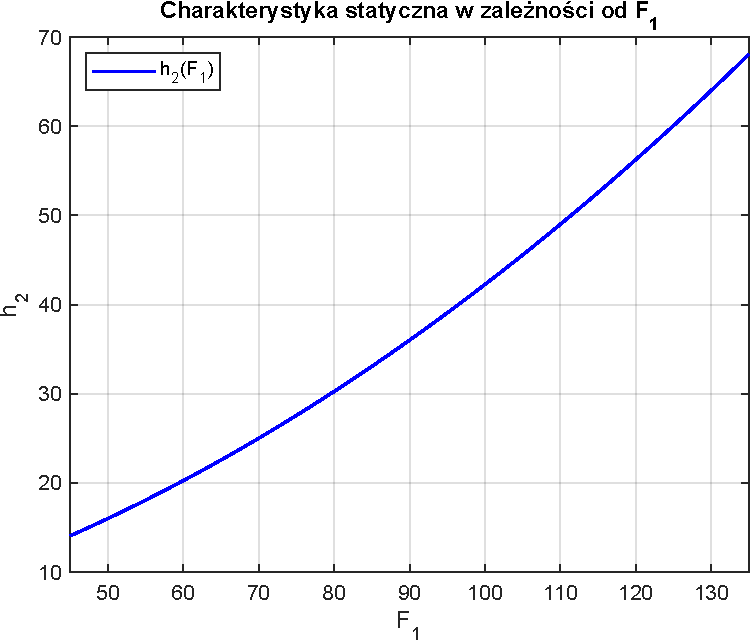
\includegraphics[width=0.8\textwidth]{pictures/static_characteristic}
\caption{Charakterystyka statyczna $h_2(F_1)$.}
\label{static_characteristic}
\end{figure}

\noindent Założono przedział zmienności sygnału sterującego w zakresie $F_1 \in [-45, 45]$.

\newpage

\section{Wymuszenia}
Po dokonaniu pierwszego kroku identyfikacji - wykreślenia charakterystyki statycznej - uzyskano wstępne informacje o obiekcie. Równania opisujące model (\ref{model_fiz}) oraz charakterystyka statyczna przedstawiona na rys. \ref{static_characteristic} pokazuje, że obiekt jest nieliniowy, stąd dokonano jego linearyzacji w punkcie pracy, tj.:
\begin{equation}
\begin{cases}
\frac{dV_1}{dt} \cong F_1 + F_D - \alpha_1 \sqrt{\frac{V_{10}}{A}} - \frac{\alpha_1}{2 \sqrt{A \cdot V_{10}}} \cdot (V_1 - V_{10})\\
\frac{dV_2}{dt} \cong \alpha_1 \sqrt{\frac{V_{10}}{A}} - \alpha_2 \sqrt[4]{\frac{V_{20}}{C}} + \frac{\alpha_1}{2 \sqrt{A \cdot V_{10}}} \cdot (V_1 - V_{10}) - \frac{\alpha_2}{4 \sqrt[4]{C \cdot V_{20}^3}} \cdot (V_2 - V_{20})
\end{cases}
\end{equation}

\noindent Linearyzacji dokonano przyjmując jako zmienną stanu objętość cieczy w obu zbiornikach. 

\begin{equation}
x = \begin{bmatrix} V_1 & V_2 \end{bmatrix}^T
\end{equation}

Następnie, podając wygenerowaną sekwencję sygnału sterującego, zbadano rozbieżność modelu liniowego i nieliniowego.

\begin{figure}[h!]
\centering
\subfloat[Wygenerowana sekwencja sygnału sterującego $u(k)$.]{
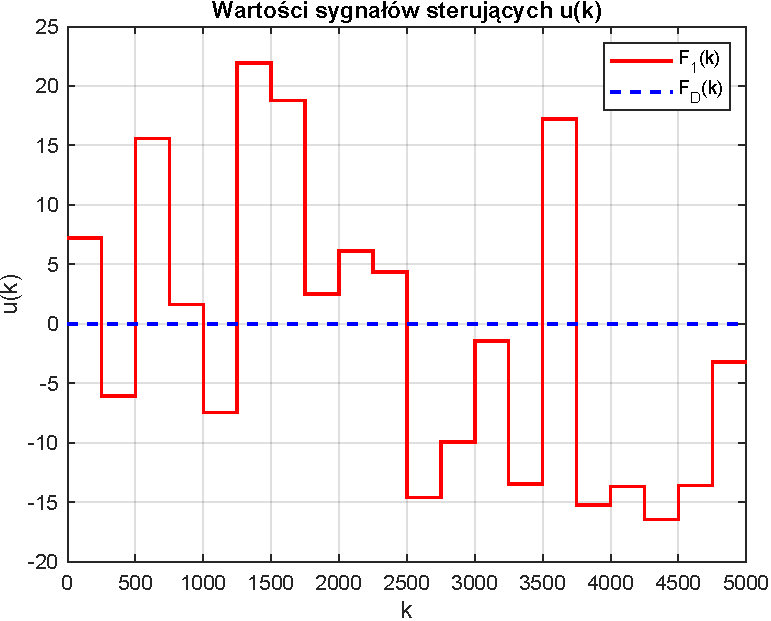
\includegraphics[width=0.45\textwidth]{pictures/u_F1}}
\hfill
\subfloat[Sygnał wyjściowy $y(k)$.]{
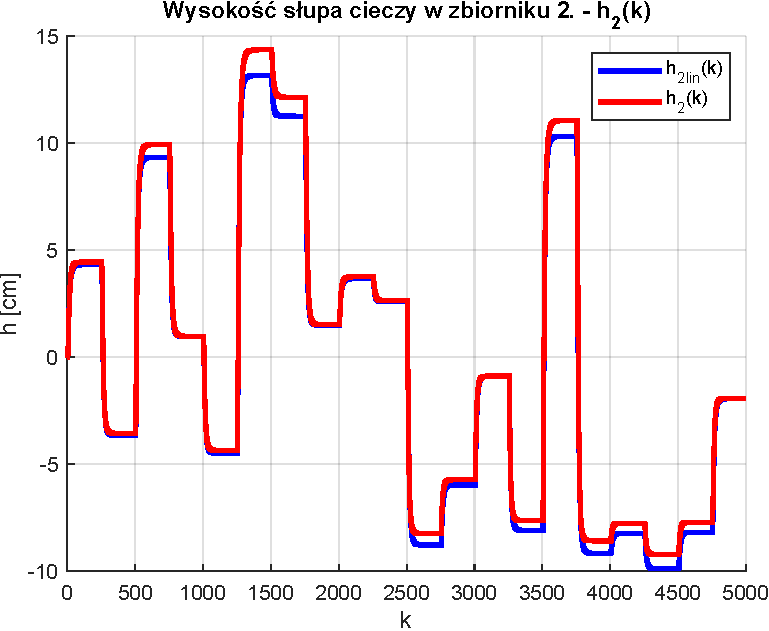
\includegraphics[width=0.45\textwidth]{pictures/y_F1}}
\caption{Porównanie modelu liniowego z nieliniowym.}
\end{figure}

Otrzymano dokładnie to czego się spodziewano. Wymuszenia nie większe niż $\pm 10 \frac{cm^3}{s}$ nie powodują znacznego wytrącenia układu z położenia równowagi, dzięki czemu model liniowy bardzo dobrze aproksymuje zachowanie układu. Niestety sytuacja pogarsza się wraz z oddalaniem się od punktu pracy - model liniowy zaczyna poważnie odbiegać od modelu nieliniowego, opisującego obiekt. W celach porównawczych policzono błędy, testując model w trybie bez rekurencji (ARX) oraz z rekurencją OE, przyjmując jako kryterium jakości błąd średni kwadratowy, tj.:

\begin{equation}
E = \sum_{k=0}^N (y(k) - y^{mod}(k))^2
\end{equation}

\noindent Wcześniej dokonano podziału wygenerowanych danych dynamicznych na dwa zbiory - uczący i~weryfikujący - stosując zasadę podziału $0\% - 50\% / 50\% - 100\%$, potrzebne do późniejszego, ewentualnego dostrajania modelu. Otrzymano następujące wyniki:

\begin{description}
\item[ARX] 
\begin{equation}
E_{ucz} = \num{0.002} \hspace{1cm} E_{wer}=\num{0.003}
\end{equation}
\item[OE] 
\begin{equation}
E_{ucz} = \num{0.470} \hspace{1cm} E_{wer}=\num{0.831}
\end{equation}
\end{description}

%\newpage

\begin{figure}[p!]
\begin{center}
\Large \textbf{Model ARX}
\end{center} 
\centering
\subfloat[Zbiór uczący.]{
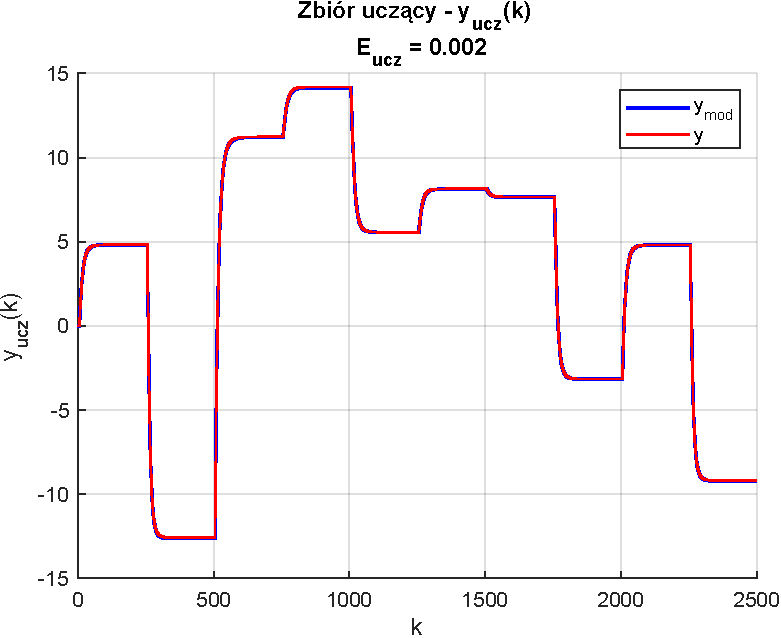
\includegraphics[width=0.45\textwidth]{pictures/arx_ucz}}
\hfill
\subfloat[Zbiór weryfikujący.]{
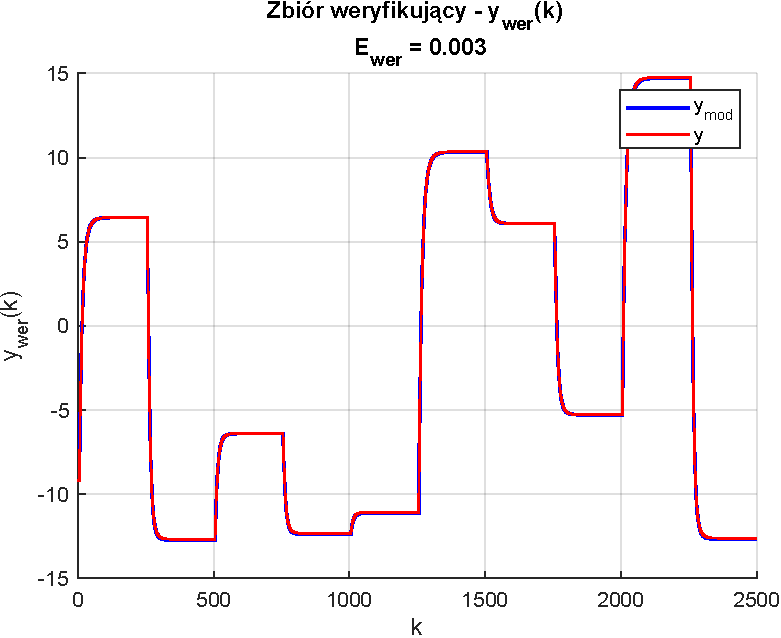
\includegraphics[width=0.45\textwidth]{pictures/arx_wer}}

\begin{center}
\Large \textbf{Model OE}
\end{center} 
\subfloat[Zbiór uczący.]{
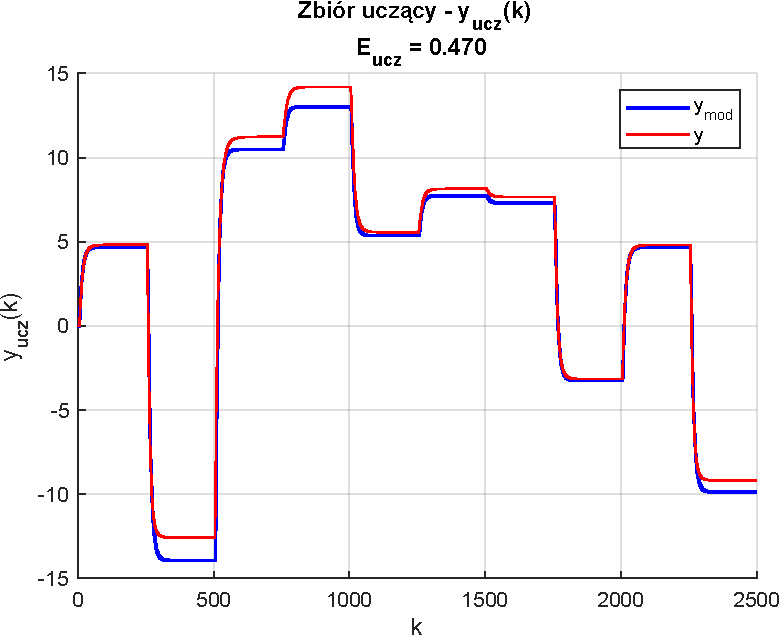
\includegraphics[width=0.45\textwidth]{pictures/oe_ucz}}
\hfill
\subfloat[Zbiór weryfikujący.]{
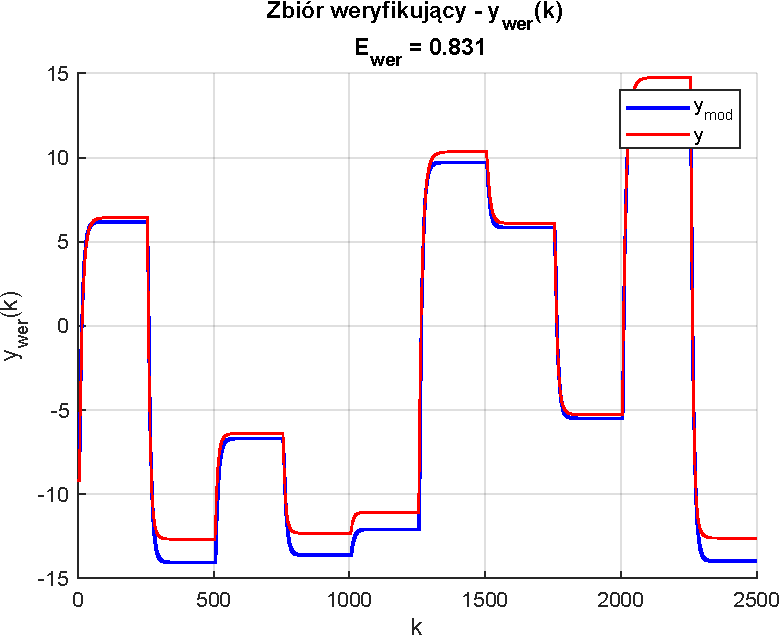
\includegraphics[width=0.45\textwidth]{pictures/oe_wer}}
\caption{Symulacja odpowiednich modeli z wykorzystaniem wygenerowanej sekwencji sygnału sterującego.}
\end{figure}

\newpage

\section{Podejście inżynierskie}
Od tej pory do dalszej analizy postanowiono przyjąć model szarej skrzynki. Informacją o~obiekcie był fakt, że układ był inercyjny. Zadano więc wymuszenie w postaci skoku jednostkowego i starano się aproksymować odpowiedź układu dobierając odpowiednie parametru dla modelu transmitancji \textit{First Order Plus Dead Time} (FOPDT), który wyraża się wzorem:

\begin{equation}
G(s) = \frac{K_0e^{-sT_0}}{T_1s + 1}
\end{equation}

\noindent Dobrane parametry:

\begin{equation}
K_0 = \num{0.6025} \hspace{1cm} T_0 = 100 \hspace{1cm} T_1 = 225
\end{equation}

\begin{figure}[h!]
\centering
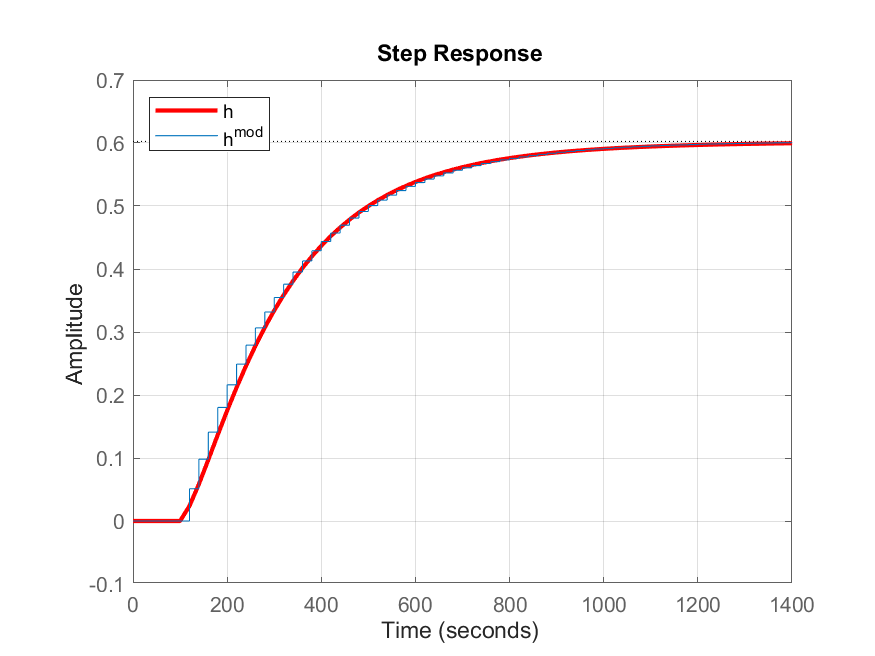
\includegraphics[width=\textwidth]{pictures/model_fopdt}
\caption{Aproksymacja odpowiedzi skokowej układu modelem FOPDT.}
\end{figure}

\newpage

Uzyskany rezultat nie był satysfakcjonujący stąd przyjęto model \textit{Second Order Plus Dead Time} (SOPDT), tj.

\begin{equation}
G(s) = \frac{K_0e^{-sT_0}}{(T_1s + 1)(T_2s + 1)}
\end{equation}

\noindent Dobrane parametry:

\begin{equation}
K_0 = \num{0.6025} \hspace{1cm} T_0 = 100 \hspace{1cm} T_1 = 212 \hspace{1cm} T_2 = 15
\end{equation}

\noindent Wynik prezentowały się następująco:

\begin{figure}[h!]
\centering
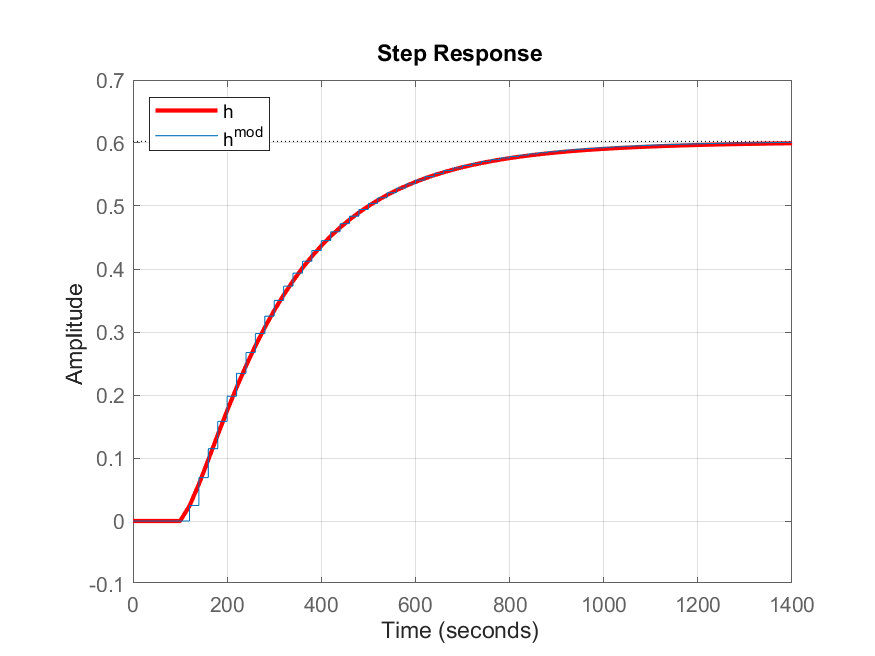
\includegraphics[width=\textwidth]{pictures/model_sopdt}
\caption{Aproksymacja odpowiedzi skokowej układu modelem SOPDT.}
\end{figure}

\newpage

Ponownie, chcąc sprawdzić skuteczność opisu obiektu regulacji wygenerowanym modelem, którego równanie różnicowe jest postaci:

\begin{equation}
\begin{aligned}
y(k) = \num{1.174} y(k-1) - \num{0.2399} y(k-2) + &\num{0.02459} u_1(k-6) + \num{0.01536} u_1(k-7) \\ 
+&\num{0.02459} u_2(k-1) + \num{0.01536} u_2(k-2) 
\end{aligned}
\label{diff_eq}
\end{equation}

\noindent wygenerowano sekwencję sygnału sterującego $u_1(k)$ oraz $u_2(k)$, który są przyrostami wartości sterujących odpowiednio $F_1$ oraz $F_D$.

\begin{figure}[h!]
\begin{center}
\Large \textbf{Model ARX}
\end{center} 
\centering
\subfloat[Zbiór uczący.]{
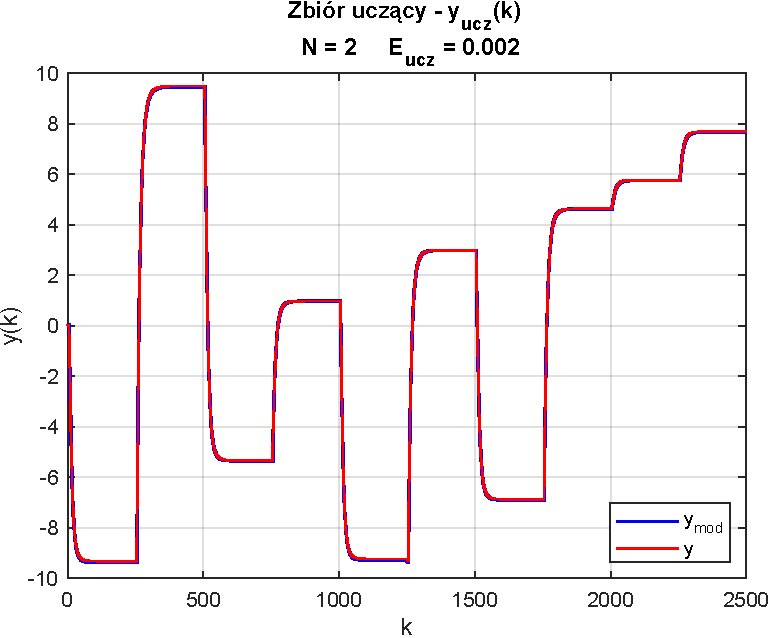
\includegraphics[width=0.45\textwidth]{pictures/arx_ucz_sopdt}}
\hfill
\subfloat[Zbiór weryfikujący.]{
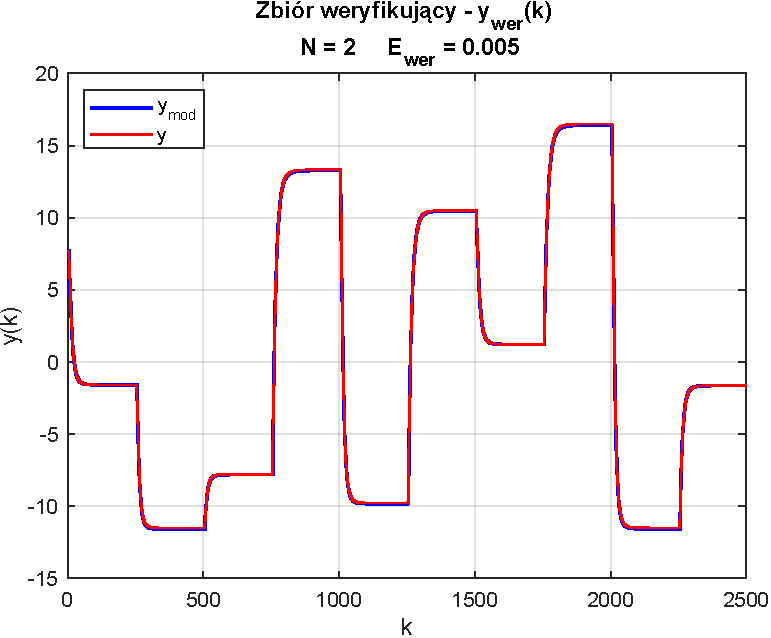
\includegraphics[width=0.45\textwidth]{pictures/arx_wer_sopdt}}

\begin{center}
\Large \textbf{Model OE}
\end{center} 
\subfloat[Zbiór uczący.]{
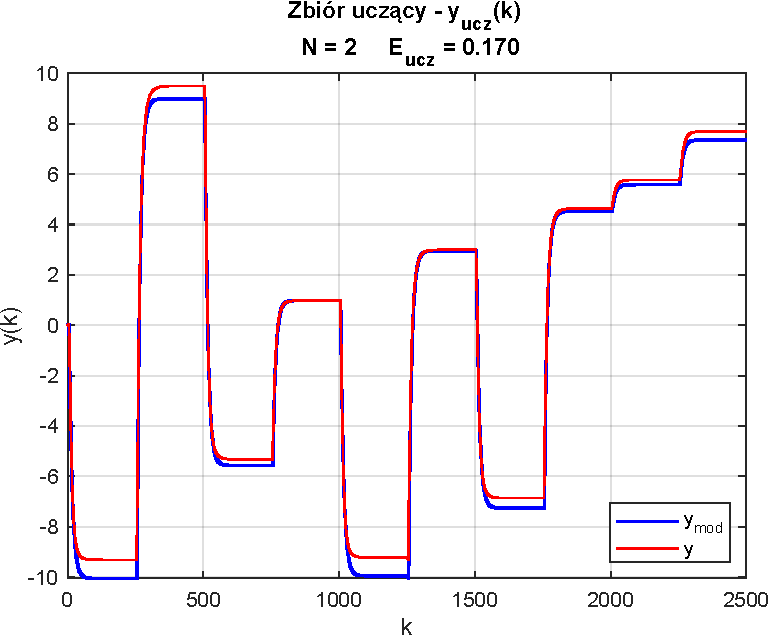
\includegraphics[width=0.45\textwidth]{pictures/oe_ucz_sopdt}}
\hfill
\subfloat[Zbiór weryfikujący.]{
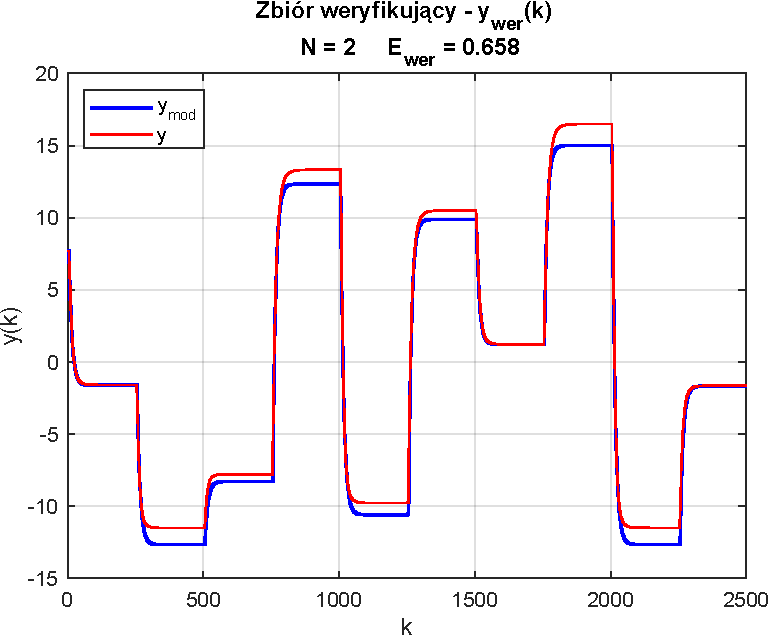
\includegraphics[width=0.45\textwidth]{pictures/oe_wer_sopdt}}
\caption{Symulacja odpowiednich modeli z wykorzystaniem wygenerowanej sekwencji sygnału sterującego.}
\end{figure}

Błędy uznano za akceptowalne na tym poziomie identyfikacji i przyjęto wyznaczony model do dalszej analizy.